\documentclass{article}
\usepackage{setspace, amssymb, amsmath, natbib, footmisc, graphicx, fontenc,
textcomp, fullpage, listings, url, booktabs}
\usepackage[T1]{fontenc}
\usepackage{lmodern}
\numberwithin{equation}{section}
\title{Term Structure Literature}
\author{Barton Baker}

\begin{document}
\doublespacing
\maketitle

\section{Introduction}
\label{sec:intro}

The relationship between the term premium on bond returns and macroeconomic
fluctuations has long been a subject of study. The causality runs in two
directions. Movements in consumption, output, inflation and monetary policy
tools impact both present and expectations of future interest rates, leading to
changes in yields all along the yield curve. Movements in interest rates on
bonds of all maturities have an impact on investment activity through their
effect on the rates that banks charge on loans to businesses and consumers. In
order to track down the theoretical underpinnings of co-movements between
macroeconomic variables and the term structure, research has begun in
consumption-based finance models and led to increasingly stylized general
equilibrium models.

Before discussing a brief history of the term structure within modern
macroeconomic economics, it is important to solidify what we mean by movements
in the term structure. The term structure of interest rates on government bonds
is often summarized by the yield curve. The yield curve is a graphical snapshot
of bond yields at a certain time, plotting yield on the vertical axis versus
maturity on the horizontal axis, with a sample of at least a few bonds.
Movements in the yield curve, come in three main forms: ``level'', ``slope'',
and ``curvature''. The level of the yield curve can be thought of as the
average yield of all the bonds. The slope of the yield curve is the difference
between the yield on any two bonds of different maturity. It common practice to
choose a very short maturity (3-month or 6-month) and a longer maturity
(greater than five years) yield to calculate the slope, as this minimizes
movements in the slope measure due to peculiarities among particular spans of
the yield curve. The curvature is the convexity of the yield curve and must be
summarized with at least 3 selected yields from the yield curve. Any
significant movements in the yield curve can be a result of the change in the
level, the slope, the curvature, or (most likely) some combination of the
three.

\section{Affine models of the term structure}
\label{sec:affine}

Affine models of the term structure are one of the primary ways through which
movements in the term structure are explained. Affine models begin with
a simple specification of the time series process governing the inter-temporal
discount factor. Adding the assumptions of no-arbitrage and the expectations
hypothesis, the entire yield curve can be derived from an affine transformation
of the process governing the discount factor\footnote{A generalized model is
derived equation by equation later in this paper.}. The use of no-arbitrage
affine models to identify movements in the term structure was first primarily
introduced in the work of \citet{vasicek1977} and \citet{coxingersollross1985},
who proposed single factor models to estimate the term structure.

With the yield curve as the empirical reference of the term structure,
empirically motivating movements in the term structure began in its modern
expression through empirical models and principal component analysis. The first
step in this direction came with \citet{nelson1987}, who proposed a three
parameter model to explain most movement in the term structure. The authors
derive a second-order differential equation that can be summarized using three
free parameters.  A linear combination of these three estimated factors
estimated over simple functions of bond maturity and a fit parameter could
explain more than 90\% of the variation in 75\% of the samples tested.
\citet{litterman1991common} reached a similar conclusion using an empirical
model of the term structure, rather than the differential equation in
\citet{nelson1987}. \citet{litterman1991common} showed that 96\% of the
movement in the term structure could be explained by three principal
components. They related these components to concepts of ``level'', ``slope'',
and ``curvature'', but remained mute on the subject of what determined these
factors and what relationship they had to observed macroeconomic variables.
Explaining what these components actually represent has been a natural jump-off
point for an entire area of research. Both papers, one from the finance
literature, one from the macro literature, while offering little in the way of
a causal explanation of the term premium, were both important catalysts for
future theoretical investigations. Specifically, these papers offered two
critical contributions to much of literature moving forward: 1) subtle
hints regarding the relationship between unobserved factors and observed yields
and 2) the number of factors needed to generate empirically meaningful yield
curves.

\citet{duffiekan1996} built-upon the affine term structure model literature by
offering a complete framework within which single-factor and multi-factor
models could be studied. Not only did this offer an opportunity to combine the
modeling framework of \citet{vasicek1977} and \citet{coxingersollross1985} with
the empirical specification of \citet{nelson1987} and
\citet{litterman1991common}, but it also served as the framework utilized by
most affine term structure model papers in its wake. \citet{duffiekan1996}
precisely derived the conditions under which a unique solution exists to affine
models and defined the general class of factor models that could be expanded to
include many factors. These models took the general form
\citep{duffiekan1996}[382]:

\begin{equation}
  R(x)=\lim_{r\downarrow{0}}\frac{-\log{f(x,\tau)}}{\tau}
  \label{duffie1}
\end{equation}

where $R$ is the short-rate, $x$ is a time-homogeneous Markov process of length
$n$ where $n$ is the number of factors influencing the term structure, $\tau$
is the maturity of a zero-coupon bond maturing at time $t+\tau$, and
$f(x,\tau)$ is the price or market value of a single zero-coupon bond of
maturity $\tau$. To solidify terminology, the short-rate in any period $t$ is
defined as:

\begin{equation}
  R(X_t)=\lim_{r\downarrow{0}}\frac{-\log{f(X_t,\tau)}}{\tau}
  \label{duffie2}
\end{equation}

\citet{duffiekan1996} assume that $X$ satisfies a stochastic differential
equation (SDE) of the form:

\begin{equation}
  dX_t=\nu(X_t)dt+\sigma(X_t)dW_t^*
  \label{duffie3}
\end{equation}

which under additional technical regularity can be expressed as a standard
Brownian motion $W$ in $\mathbb{R}^n$:

\begin{equation}
  dX_t=\mu(X_t)dt+\sigma(X_t)dW_t
  \label{duffie4}
\end{equation}

Equations \ref{duffie1}, \ref{duffie2}, and \ref{duffie4} define what
\citet{duffiekan1996} call ``General Factor Models'' of the term structure.
Beyond this broad categorization of factor models, \citet{duffiekan1996} show
affine factor models satisfy the requirements of the system outlined above.
They define a class of compatible models by specifying the functional form of
$f(x,\tau)$:

\begin{equation}
  f(x,\tau)=\exp[A(\tau)+B(\tau)\cdot{x}] 
  \label{duffie5}
\end{equation}

where $A$ and $B$ are $C^1$ functions on $[0,\infty]$. This is the form that
affine models have taken in the main thread of affine term structure model
literature.

In addition to laying out this formative framework, the self-proclaimed primary
purpose of \citet{duffiekan1996}, \citet{duffiekan1996} also offered
a suggestion for a solution method to these models, particularly pertinent in
the case of multiple factors. This method involved first solving for elements
of $B$ from Eq. \ref{duffie5} using the fourth-order Runge-Kutta method.
Following this initial parametrization of $B$ a combination of Newton-Raphson
and ADI solution algorithms are applied to match an increasing number of
consistency conditions. While this exact method is not always used in modern
affine model term structure models, the approach of iteratively estimating
different parameters in different rounds has become very popular \footnote{In
fact, the Kalman filter is the only other solution method that is widely used
to solve these models}. The exact method prescribed by \citet{duffiekan1996}
becomes increasingly untractable with higher numbers of factors. Estimation
methods for affine term structure models are treated as a whole in
\citet{duffee2004estimation}. Given that a number of estimation methods had
become popular in the early 2000's, the authors examined Maximum Likelihodd
(ML), Estimated Method of Moments (EMM), and a Kalman filter method. They find
that the ML and EMM method does not perform well under highly-persistent, small
samples common in bond data. Specifically, the ML method results in biased
parameter estimates in the speed of mean reversion
\citet[19]{duffee2004estimation}, but overall efficient use of the information
when feasible. At the time of writing, ML methods were computationally
intensive for affine term structure models. The EMM method performs much worse
than the ML method, resulting mostly from the differences in the curvature of
the auxiliary function between the highly-persistent small sample and the true
parameter function of the hypothetical infinite sample. The Kalman filter
method results in less precision than ML estimates (higher standard deviations
of the estimates under Monte Carlo techniques), but is more feasable than ML
techniques, where searches over a very large parameter space can become
computationally intensive.

By building the sandbox within which the affine-model term structure literature
could grow, \citet{duffiekan1996} spurred a flurry of papers integrating both
latent and observed factors to estimate the term structure. Because these
models relied on no-arbitrage assumptions and a single pricing kernel, the
implied term premium could easily be computed post-estimation by attributing
any yield on longer-maturity bonds above and beyond the implied risk-free yield
to the term premium. Much of this work has exclusively used unobserved latent
factors to estimate the term structure while others have combined observed
macro variables with latent variables, with even others using exclusively
observed macro variables as factors. Latent variables are unobserved components
of a statistical process that are derived using regression methods, unlike the
components the estimated components in Principal Component Analysis (PCA) which
are always orthogonal. Major investigations using exclusively latent factors
include \citet{daisingleton2000} and \citet{kim2005arbitrage}. While
\citet{daisingleton2000} are able to fit the observed moments of the term
structure quite well, their use of latent factors offer little in the way of
theoretical interpretation. The model proposed in \citet{kim2005arbitrage},
a three latent factor affine model of the term structure has became the
workhorse model for generating a reliable estimate of the term premium.
\citet{kim2005arbitrage}'s main advantage over \citet{daisingleton2000} is that
they take into account the examination of estimation methods performed in
\citet{duffee2004estimation}, using a small sample consistent Kalman filtering
to estimate their model.\citet{daisingleton2000} instead use a simulated method
of moments method requires more identifying restrictions on the model
parameters. 

In response to criticisms that unobserved latent factors offer little in the
way of causal relevance, the \citet{ang2003no} extension of
\citet{daisingleton2000} uses two macro variables, inflation and real activity,
and three latent factors, per the suggestion of \citet{litterman1991common} and
\citet{nelson1987}. They find that the addition of observed macro factors
significantly increases the ability of the model to forecast term structure
moments. This paper showed that observed macro variables could be used to
summarize at least some of the information entering expectations formation
related to movement in the term structure.  \citet{sack2005monetary} took this
approach one step further in their attempt to estimate the effects of
zero-lower bound restricted alternative monetary policy.
\citet{sack2005monetary} used five observable macro variables\footnote{The
  details of which are discussed in section \ref{sec:repl}.} 
as their factors, arguing that their five variables summarized the relevant
information set entering bond pricing decisions. They find that their model is
able to fit the yield data relatively well, with pricing errors increasing with
maturity (see Table \ref{tab:1} for details) and realistic tracking of
the paths of yields at all maturities included in the analysis (see Figure
\ref{fig:bern_fig1}). \citet{rudebusch2008macro} (originally appearing in 2004
as \citet{rudebusch2004macro}) also integrated both latent and observed factors
into an affine model as in \citet{ang2003no}, but instead related the observed
factors to the latent factors through New Keynesian structural relationships
rather than direct inclusion in the information set.
\citet{rudebusch2008macro} showed that including the macro variables added to
the model fit, but including the observed factors did not change the estimates
of the unobserved factors by much.  \citet{diebold2006macroeconomy} provided an
interesting link between non structural affine models of the term structure and
the New Keynesian general equilibrium framework. With the exception of
\citet{rudebusch2008macro}, the other affine models mentioned only allowed for
causality in the direction of macro and latent factors to term structure
yields.  \citet{diebold2006macroeconomy} relates the first two latent factors
to observed macroeonomic outcomes. The first latent factor or ``level'' factor
is related to inflation, while the second factor or ``slope'' factor is related
to capacity utilization or cyclical fluctuations.
\citet{diebold2006macroeconomy} attempts to focus on this issue of
bi-directional causality, finding that while both directions are significant,
the effect of macro and latent factors on term structure moments are much more
important than the effect of term structure moments on macro and latent
factors.

In addition to combining observed and unobserved factors to increase ability of
affine models to explain the term structure, other modeling methods have been
attempted to supplement or refine the information available to
price-determining bond investors. \citet{kimorphanides2005} proposed that the
three-factor model can be supplemented with Blue-Chip survey estimates of
6-month- and 12-month-ahead expected 3-month T-bill yield in order increase the
ability of the model to fit the data. The authors show that the survey
forecasts add important information to the model solution algorithm, decreasing
the required sample size for stable parameter estimates, allowing estimation to
take place using shorter periods where the condition of stable ``true''
parameters is more likely to hold. \citet{orphanideswei2010} took a different
approach, echoing the approach of \cite{orphanides2001monetary} to increase the
fit of a Taylor-rule using real-time data and adding the possibility of
time-varying parameters. Instead of beginning with an unobserved latent factor
model, \citeauthor{orphanideswei2010} compare several versions of affine term
structure models, but their final proposed model is where affine model
state-space parameters are iteratively estimated over time using VAR(2) with
real-time data available at time $t$. While the authors show that a 3 factor
affine model still outperforms their proposed model, the model iteratively
estimated with real-time data outperforms their baseline comparison model,
which is estimated using final data and without the possibility of time-varying
parameters. Little time was spent in this paper on examining the advantage of
using real-time data to estimate structural models, since the focus was more on
using an iterative VAR to inform the pricing kernel.

All affine models of the term structure can be built up from a basic general
setup. The rest of this section examines the set-up and estimation strategies.

Affine models of the term structure begin with the assumption that the pricing
kernel for all government bond yields is completely determined by an VAR
process, most often summarized as a VAR(1) for simplicity\footnote{This
  notation is taken from \citet{sack2005monetary} and \cite{ang2003no}, but
expanded to refer to a broader class of models}:

\begin{equation}
    X_t = \mu + \Phi{X_{t-1}}+\Sigma\varepsilon_t
    \label{eq:aff1}
\end{equation}

where $X_t$ is an $n\times1$ vector of latent unobserved and/or observed macro
factors. Eq. \ref{eq:aff1} fully identifies the time series of the information
entering bond pricing decisions and $\varepsilon$ is assumed
$\mathcal{N}(0,1)$.

The price of any $n$-period zero-coupon bond in period $t$ can be recursively
defined as the expected product of the pricing kernel in period $t$, $m_t$ and
the price of the same security matured one period in $t+1$:

\begin{equation}
    p_t^n=E_t[m_{t+1}p_{t+1}^{n-1}]
    \label{eq:aff2}
\end{equation}

We assume that the period-ahead pricing kernel is conditionally log-normal,
a function only of the current risk-free rate, $i_t^{(1)}$ and the prices of
risk, $\lambda_t$:

\begin{equation}
    m_{t+1}=\exp{(-i_t^{(1)}-\frac{1}{2}\lambda_t'\lambda_t-\lambda_t'\varepsilon_{t+1})}
    \label{eq:aff3}
\end{equation}

Without perfect foresight, agents price risk attributed to each macro factor
given the current state-space, $X_t$:

\begin{equation}
    \lambda_t = \lambda_0 + \lambda_1X_t
    \label{eq:aff4}
\end{equation}

where $\lambda_0$ is $n\times1$ and $\lambda_1$ is $n\times{n}$.

We can then define the price of any zero-coupon bond of maturity $n$ in period
$t$ as a function of the pricing kernel, combining Eqs. \ref{eq:aff2} and
\ref{eq:aff4}:

\begin{equation}
    p_t^n=\exp{(\bar{A}_n+\bar{B}_n'X_t)}
    \label{eq:aff5}
\end{equation}

where $\bar{A}_n$ and $\bar{B}_n$ are recursively defined as follows:

\begin{eqnarray}
    \bar{A}_{n+1}=\bar{A}_{n}+\bar{B}_n'(\mu-\Sigma\lambda_0)+\frac{1}{2}\bar{B}_n'\Sigma\Sigma'\bar{B}_n'-\delta_0  \nonumber \\
    \bar{B}_{n+1}'=\bar{B}_n'(\Phi-\Sigma\lambda_1)-\delta_1'
    \label{eq:aff6}
\end{eqnarray}

with $\bar{A}_1=\delta_0$ and $\bar{B}_1=\delta_1$ and $\delta_0$ and
$\delta_1$ relate the macro factors to the one-period risk free:

\begin{equation}
    p_t^1=\exp{\delta_0+\delta_1X_t}
    \label{eq:aff7}
\end{equation}

In the same way, the yield can be expressed as:

\begin{equation}
    y_t^n=A_n+B_n'X_t
    \label{eq:aff8}
\end{equation}

where $A_n=-\bar{A}_n/n$ and $B_n=-\bar{B}_n/n$.

In the case where $X_t$ contains only observed macro-variables, $\mu$, $\Phi$
and $\Sigma$ are easily calculated using ML in first stage of the estimation
process. In the second stage, Eq. \ref{eq:aff8} is fit to various points along
the yield curve also using ML or Least Squares. This second stage estimation
becomes especially trivial if the risk free rate is included in the set of
macro-variables informing bond pricing decisions, $X_t$. This is the method
used (with Least Squares) in \citet{sack2005monetary}.

When unobserved latent variables are included in $X_t$, the solution algorithm
becomes more complicated. One method to solve for the unknown factors has been
to assume that a number of points on the yield curve, equal to the number of
unobserved latent factors, are observed without error. The factors are first
solved for using the yields measured without error and the likelihood function
of the VAR system and then the remainder of the yield curve is estimated by
maximizing the likelihood of the yield curve relationship, Eq. \ref{eq:aff8}.
Practitioners usually choose well-spaced points along the yield curve (3-month,
12-month, and 36-month yields), but these choices are mostly arbitrary.
\citet{ang2003no} utilizes this method.

Another method of estimating the affine system is by using the Kalman filter.
The VAR(1) system defined by Eq. \ref{eq:aff1} and the yield/macro factor
relationship of Eq. \ref{eq:aff8} together naturally define a state-space
system. The system can then be iteratively solved using standard Kalman filter
solution algorithms. This method has become more popular in affine term
structure model papers in recent time, since it was first compared to ML
methods in \citet{duffee2004estimation} and utilized in the benchmark latent
factor model of \citet{kim2005arbitrage}.

\section{Replication of \citet{sack2005monetary}}\label{sec:repl}

This section is an attempt to replicate the results of
\citet{sack2005monetary}, an investigation into the effects of alternative
monetary policy when a zero-lower bound for the short-rate is a binding
condition. The second section of their paper involves the estimation of an
affine model of the term structure using five observed factors: an HP-filtered
employment gap, inflation over the past year (measured as PCE excluding food
and energy), expected inflation over the subsequent year from the Blue Chip
survey, the federal funds rate, and the year-ahead Eurodollar rate. This is the
section that this small paper will attempt to replicate. They utilize a VAR
directly estimated on the five macro variables to generate a pricing kernel to
fit the implied zero-coupon bonds (CRSP Fama files) of maturities six-months
and one, two, three, four, five, seven and ten years. They use monthly data
from 1982 to 2004. While the authors do not present the exact parameters
estimates, they do present graphs of the two-year and ten-year actual,
predicted, and risk neutral yields on bonds. They also present prediction
errors for all of the yields used to estimate the model, using an estimated
model with the Eurodollar and without.

Presented in Figure \ref{fig:bern_fig1} are the two graphs presented as they
appear in \citet{sack2005monetary}[46]. Each graph shows three lines: the
actual yield, the model-predicted yield, and the risk-neutral yield. The
model-predicted and risk-neutral yield are both generated from the estimated
parameters, the difference between which is the implied term premium. 

\begin{figure}[htp]
  \begin{center}
    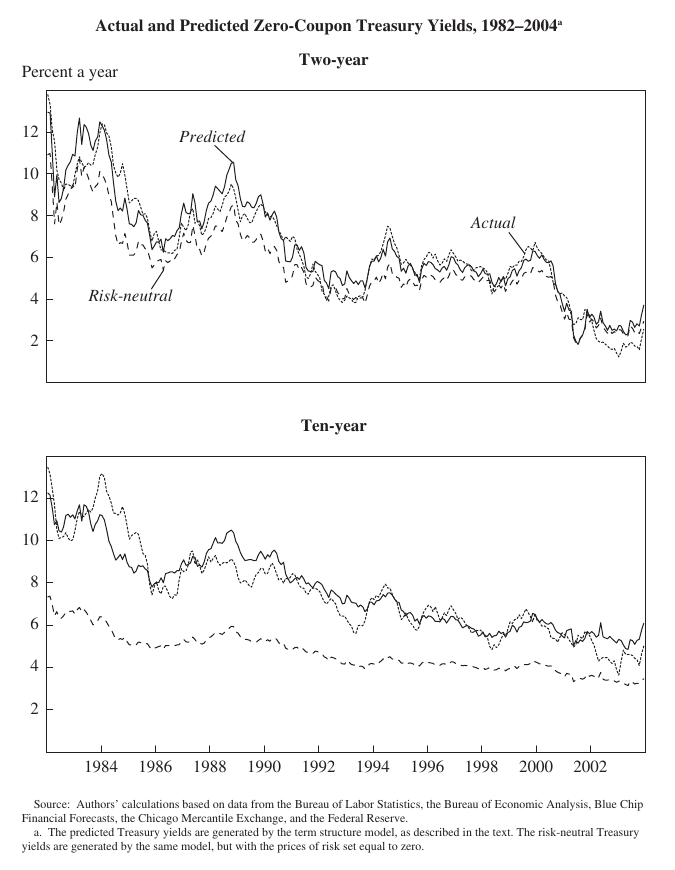
\includegraphics[scale=0.6]{./figures/bern_fig1.png}
  \end{center}
  \caption{Page 46 from \citet{sack2005monetary}}
  \label{fig:bern_fig1}
\end{figure}

Table \ref{tab:1} is also taken from \citet{sack2005monetary}[47],
presenting the pricing errors for all of the yields used for estimating using
two models, with and without Eurodollar futures as a macro factor.

\begin{table}[htp]
  \begin{center}
    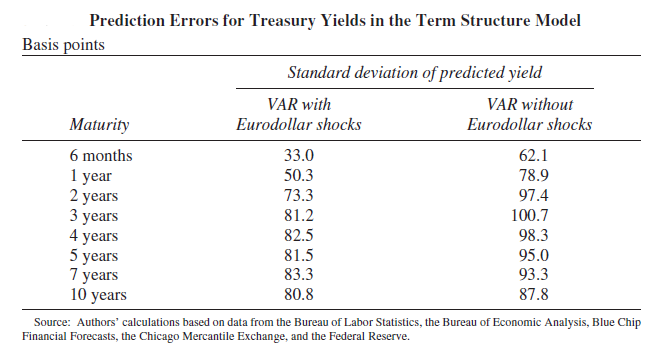
\includegraphics[scale=0.6]{./figures/bern_fig2.png}
  \end{center}
  \caption{Page 47 from \citet{sack2005monetary}}
  \label{tab:1}
\end{table}

As a proof of concept, this paper attempts to replicate the results presented
in \citet{sack2005monetary} (BSR) using a custom-written solution method in
Python (see accompanying code-base) and using data as close as possible to data
used in BSR. Instead of 1982 to 2004, this replication used data from December
1987 to December 2004 because of data availability. Instead of Blue Chip survey
inflation year-ahead forecasts, expected annual inflation from the Survey of
Consumers \citet{mich} is used as an indicator of inflation expectations. The
other VAR factors are as in BSR. Also, because of current unavailability of
Fama-CRSP implied zero-coupon yields on Tresuries, Treasury Constant Maturities
available from FRED are used as a second-best replacement \citet{fred} and the
4 year maturity Tresuries are not included.

The parameters governing the prices of risk are estimated by minimizing the sum
of squared predictions errors. Using these parameter estimates, the
model-predicted yields are generated by feeding the VAR elements, $X_t$ for
each $t$ into Equation \ref{eq:aff4} using the estimated $\lambda_0$ and
$\lambda_1$. By setting the prices of risk to zero in $\lambda_0$ and
$\lambda_1$, the implied risk-neutral yields can be generated. These two time
series, along with the actual yields are presented graphically in figures
\ref{fig:repl1} and \ref{fig:repl2}, echoing their presentation Figure
\ref{fig:bern_fig1} from BSR.

\begin{figure}[htp]
  \begin{center}
    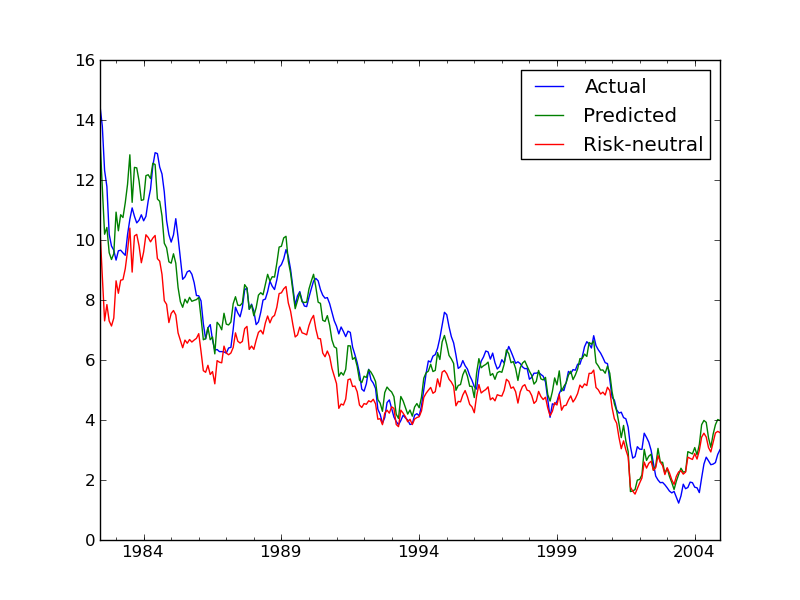
\includegraphics[scale=0.6]{./figures/twoyr_rep.png}
  \end{center}
  \caption{Author's estimation results of 2-year Treasury Constant Maturity}
  \label{fig:repl2}
\end{figure}

\begin{figure}[htp]
  \begin{center}
    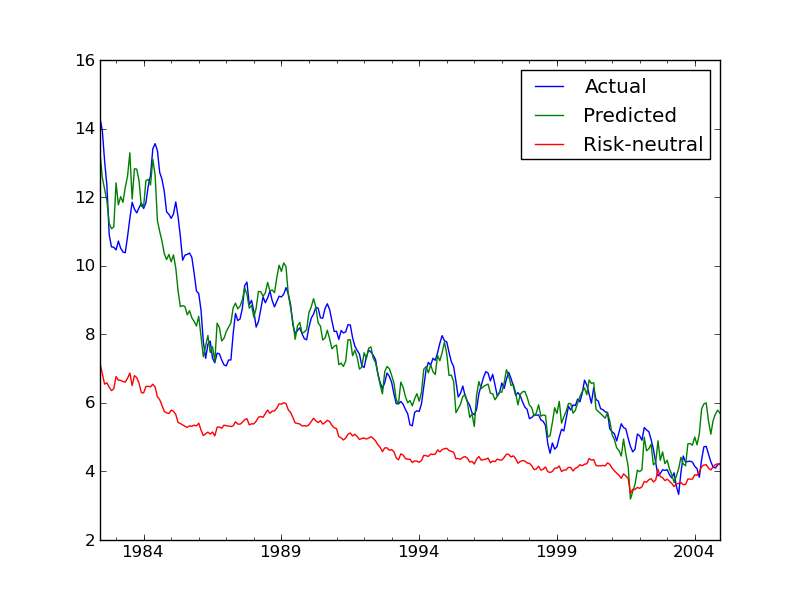
\includegraphics[scale=0.6]{./figures/tenyr_rep.png}
  \end{center}
  \caption{Author's estimation results of 10-year Treasury Constant Maturity}
  \label{fig:repl1}
\end{figure}

As you can see, the estimates do not match exactly, but this can most likely be
attributed to non-matching data sources. The results qualitatively match in
a few ways. The estimation results in smaller pricing error for the two year
maturity yields compared to the ten year. This is probably a result of the fact
that the federal funds rate is included as a factor in the VAR and the
shorter-term maturity bonds are more likely to be directly effected by
movements in the federal funds rate. Also, as in BSR, the replication obtains
the appealing result that the term premium, the distance between the predicted
and risk-free yields, increases with maturity.

The pricing errors for the replication models with and without Eurodollar (ED)
futures are presented in Table \ref{tab:2}. While the pricing errors do not
exactly match the results from BSR presented in Table \ref{tab:1}, they do
emulate two of the generate characteristics present in the BSR results.
Firstly, the smallest pricing error in both the no-ED and ED model is with for
the 6 month maturity yield. This is not surprising as the VAR system has more
direct information to inform the pricing kernel at this end of maturity
spectrum given its inclusion of the federal funds rate. Secondly, the inclusion
of Eurodollar futures does reduce the pricing error for Treasury yields of all
maturities in both the original BSR model and this replication.

\begin{table}
\begin{center}
\begin{tabular}{|c|c|c|}
    \hline
    \textbf{Maturity} & \textbf{VAR with ED shocks} & \textbf{VAR without ED
    shocks}\\ \hline
    6 months  & 17.1 & 18.3 \\ \hline
    1 year    & 21.8 & 25.1 \\ \hline
    2 years   & 24.6 & 34.6 \\ \hline
    3 years   & 23.3 & 36.7 \\ \hline
    5 years   & 21.4 & 37.3 \\ \hline
    7 years   & 19.8 & 34.4 \\ \hline
    10 years  & 20.0 & 33.4 \\ \hline
\end{tabular}
\end{center}
\label{tab:2}
\caption{Pricing error in basis points}
\end{table}

Parameters

\begin{table}
  \centering
  \begin{tabular}{lcrrrrr}
    %row-major order for output
    \toprule
    & $\lambda_0$ &\multicolumn{5}{c}{$\lambda_1$} \\
    \cmidrule{2-2} \cmidrule(l){3-7} \\
    &  & Empl. Gap & Inflation & Exp. Inflation & Fed. Funds
    & Euro-Dollar Fut. \\
    Empl. Gap       & 13605.3199    &-19532.194 &-777.9469 &592.7662
                    &36547.055 &-3989.245 \\
                    & (87417.1363)  &(916243.4202) &(3444.2113) &(2989.3648)
                    &(53123.5917)   &(3704.0872) \\ %this row is for std errs
    Inflation       &  148.2248     &3429.2952 &26.4911 &18.8169 &-290.9901
                    &23.1623 \\
                    & (553.6984)    &(8548.1197) &(43.1522) &(23.2349)
                    &(225.6018) &(50.48) \\
    Exp. Inflation  &  4.8861       &-200.1545 &-1.9348 &-2.2384 &86.8642
                    &-9.2543 \\
                    & (192.732)     &(2199.7329) &(9.499) &(6.6299) &(90.9963)
                    &(9.466) \\
    Fed. Funds      & -16.1298      &-89.8569 &-2.1435 &0.1829 &3.4266
                    &0.3604\\
                    & (13.289)      &(406.1849) &(2.185) &(1.4263) &(26.4616)
                    &(2.7115) \\
    EuroDollar Fut. &   -30.9481    &-187.8645 &0.3971 &-1.9902 &-44.3954
                    &4.215 \\
                    & (116.5332)    &(1191.8426) &(4.2237) &(4.1643) &(86.4603)
                    &(4.9276) \\
    \bottomrule
  \end{tabular}
  \caption{Parameter estimates with standard errors in parenthesis. Only those
  parameters that were not set to 0 are displayed.}
  \label{tab:3}
\end{table}

\section{moving forward}

\subsection{real-time data and affine models of the term structure}

At this point, my dissertation would break into three chapters, all related to
affine models of the term structure.

Chapter 1 will first replicate the results of \citet{sack2005monetary} (BSR),
using the identical data sources to approach their results as close as
possible. After these results are replicated, the data will be extended to up
the financial crisis and after the financial crisis to see if the pricing error
increases or decreases. It is likely that the pricing error would deteriorate
by extending the data into the crisis period, since there is no inclusion of
a high-frequency indicator of uncertainty. To respond to this deterioration,
one of the factors (likely the Eurodollar futures) will be replaced with an
aggregate measure of credit default swaps. My hypothesis is that including this
factor will lead to lower pricing error for affine models during crisis
periods. This analysis for this chapter will largely build off of the analysis
presented in the above section.

Chapter 2 will focus on improving the information set feeding bond pricing by
using real-time rather than final macro-data. The aim of this chapter will be
to answer the question: Does real-time data increase the fit of affine models
of the term structure that use observed factors? While real-time data has been
integrated into an affine model framework in \citet{orphanideswei2010}, the
focus of the paper was not on the value-added of using real-time data. Because
the definition of the pricing kernel at time $t$ is supposed to reflect all
information informing bond pricing decisions at time $t$, the necessity of
adding unobserved latent factors to an affine model with observed factors is
most often to increase the fit of the model, because the observed factors alone
cannot match all of the variation. This may simply be an artifact of
incorrectly attributing available information regarding macroeconomic
fundamentals at time $t$. Final versions of data, especially GDP and inflation,
are often not available until quarters after the period that they refer to,
making final data insuitable as a proxy for available information at time $t$
influencing bond pricing decisions at time $t$. 

This will require some theoretical derivation of the exact advantage of using
real-time data vs. final-data in estimating term structure models. After
deriving this advantage, I will estimate models using both real-time and final
data from a variety of samples of U.S data and compare the two to estimate
where the gain in explanatory value is statistically significant.
\citet{orphanideswei2010} show that estimating the model using real-time data
and time-varying parameters results in overall lower estimates of the term
premium, because a higher proportion of the premium can be attributed to future
short-rate expectations. I will compare my results to the results presented in
\citet{orphanideswei2010} in order to place this chapter in the affine term
structure model literature.

Chapter 3 will be a computational extension of the Python model solving class.
In this chapter, I will write a C++ extension to the python class that I have
already written that solves latent factor affine models of the terms structure.
After reading through the solution methods suggested in
\citet{daisingleton2000}, \citet{ang2003no} and \citet{duffee2004estimation},
it seems as though some of the assumptions needed to solve these models are
largely arbitrary. For example, because of the large number of free parameters
in the model presented in \citet{ang2003no}, the authors have to assume that
certain parameters are equal to 0 after they are insignificant at the 5\% level
and iterate over multiple steps where structural and price of risk parameters
are estimated one after the other. Because of how arbitrary this seems, I'd
like to investigate the implications of slightly altering their approach on the
qualitative results.

It may be interesting to see if the affine model produced measure of the term
premium referenced in many of the post-crisis papers results in a much lower
proportion of the term premium explained by the portfolio balance channel
rather than through expectations of future short-term interest rates (as in
\citet{bauerrudebusch2011}). because using final data may result in
a mis-specified affine model, the percentage of the change in yields on
longer-maturity bonds may be incorrectly split between a term premium component
and expected future short-rates.

I would also like to address the conclusion of \citet{diebold2006macroeconomy}
using real-time data. because \citet{diebold2006macroeconomy} uses the same
data on both sides of the causality (term structure causing macroeconomic
fluctuations and vice versa), it would be interesting to see if their model would
generate the same conclusions of 1) interest rates $\rightarrow$ macro factors
is not as important as 2) macro factors $\rightarrow$ interest rates if the
macro factors in 1) are replaced with real-time macro data.

\subsection{Work that I have done}

I have already written a maximum likelihood solver in Python for models and
have used it for a previous term paper. I would like to fully utilize it and
also move onto a Kalman filter approach to estimating the system. I've also
worked through solving some of the DSGE models of the term premium addressed in
section \ref{sec:struct} using the permutation solution algorithm proposed by
\citet{swanson2006higher}.

\section{Structural models of the term structure}\label{sec:struct}

This section is not as relevant as before. Moving forward, I will be focusing
exclusively on affine models of the term structure for my own investigation,
but will use the results in reached in DSGE models of the term structure as
a reference for how affine models of the term structure fare computationally,
statistically,  and structurally within the broader realm of models of the term
structure.

While affine models of the term structure offer a rigorous way of explaining
movements in the term structure, the framework offers little in the way of
microeconomic foundations or structural interpretations. Given this, an entire
parallel literature attempting to model movements in the term structure of
interest rates with structural macroeconomic models has grown. This literature
has progressed in a way where a series of issues are dealt with in matching
structural models to the data. Even though \citet{mehraprescott1985} focused on
the equity premium, rather than the term premium, the insight of their paper
held just as important to the term premium literature: the risk aversion
parameter plays a primary role in determining the differential yields among
securities, and in order to fit the yields on equity, estimates of this
parameter are way beyond any reasonable microeconomic estimates. This
observation became a vital crux of the consumption based models of the term
structure in 1990s. \citet{donaldsonetal1990}, using a popular
consumption-based model with power preferences, showed that the simple model
even with huge shocks to consumption was incapable of generating the real term
structure. Expected utility in this model, along with the other
consumption-based models of the 1990s, took the following form:

\begin{equation}
  E_t(\sum_{t=0}^\infty{\beta^t\frac{c_t^\gamma-1}{\gamma}})
  \label{eq1}
\end{equation}

where $\beta$ is the inter-temporal discount factor, $c_t$ is consumption in
period $t$, and $\gamma$ is a parameter.

The functional form of expected utility ends up playing a key role in
determining the ability of structural models' to generate a sizeable term
premium. Reinforcing \citeauthor*{donaldsonetal1990} conclusion,
\citet{denhaan1995} showed in order to generate a sizeable term premium in this
simple consumption model, persistent expected growth rates of consumption and
negative autocorrelation of consumption growth are required. Neither of these
are present in the U.S data. Without these characteristics, the standard
consumption model results in a negative sloping yield curve.

One of the first papers to offer an innovation as a possible way of generating
a sufficient asset price premium was \citet{campbellcochrane1999}. While this
paper intended to explain the equity premium, the same function form was
adopted by much of the following term premium literature. The driving
innovation in this paper was the introduction of a habit to the utility
specification:

\begin{equation}
  E_t(\sum_{t=0}^\infty{\beta^t\frac{(c_t-X_t)^(1-\gamma)-1}{1-\gamma}})
  \label{eq2}
\end{equation}

where $X_t$ is the habit.

Because the representative agent derives utility from some value over and above
some baseline value, the habit, agents aim to smooth consumption, resulting in
a more persistent consumption stream compared to the standard power utility
specification (Eq.~\ref{eq1}). Smoother consumption results in equity prices
that are correlated with movements in consumption relative to the habit
parameter, making them more risky, thus requiring a higher return in
compensation for that risk. This lessens the necessity of an excessively high
risk aversion parameter. Even though \citeauthor{campbellcochrane1999} were
able to match the empirical equity premium using this method, they still
required a very high steady state risk aversion. 

\citet{jermann1998} moves the innovations of the above mentioned
finance-consumption models into a general equilibrium, real business cycle
(RBC) framework. Attempting to price both equity and bonds,
\citeauthor{jermann1998} utilizes both a utility specification with habit and
capital adjustment costs to fit movements in equity and bond yields. Although
\citeauthor{jermann1998}'s model results in a short-term interest rate that is
much too volatile, risk-premia on bonds that are too high relative to the
equity premium, and very low consumption volatility, his integration of
structural rigidities into a general equilibrium framework was an important
step in the development of empirically binding micro-founded term structure
models.

The importance of habit is further investigated in a complete general
equilibrium model in \citet{lettauuhlig2000}. On top of consumption habit to
generate meaningful term premia, \citeauthor{lettauuhlig2000} attempt to
overcome empirically unsupported steady consumption by introducing labor habit.
\citeauthor{lettauuhlig2000} hypothesize that volatility in labor is drawing
volatility away from consumption, but applying the habit in labor habit on top
of habit in consumption results in much smoother labor paths, but still
relatively steady consumption paths. Altering other parameters are unable to
increase consumption volatility without lessening model fit of other
macroeconomic variables. \citeauthor{lettauuhlig2000} does not attempt to fit
the model to asset yield data (bonds or equity), but the purpose of the paper
echoes the importance of consumption in the general equilibrium asset price
literature, leaving many remaining questions for habits empirical tenability.
\citet{boldrinetal2001} takes a similar approach in a general equilbrium
framework, introducing inter-sectoral rigidities rather than labor habit, but
is still left with consumption processes that are too persistent to match to
the data.

Following the seeming inability of general equilibrium models with consumption
habit utility specifications to generate empirically tenable consumption
streams, the structural term premium literature turned to other utility
specifications. The most fruitful of these forays has been the introduction of
preferences a la \citet{epsteinzin1989} (EZ). In both the power utility
(Eq.~\ref{eq1}) and habit-adjusted power utility (Eq.~\ref{eq2}) cases,
a single parameter ($\gamma$) determines both the elasticity of inter-temporal
substitution (EIS) and the within period level relative risk aversion (RRA).
EZ preferences enter these DSGE models in the form: 

\begin{equation}
  V_t = u(c_t,l_t) + \beta(E_tV_{t+1}^{1-\alpha})^{1/(1-\alpha)}
  \label{eq3}
\end{equation}

with:
\begin{equation*}
  u(c_t,l_t)\equiv\frac{c_t^{1-\phi}}{1-\phi}
\end{equation*}

where $V_t$ is utility in period $t$ and $\alpha$, $\phi$, $\chi_0$, and $\chi$
are parameters.

The key difference, both theoretically and for matching to empirical
distributions, is that the parameter governing EIS, $\alpha$, is distinct from
the parameter governing relative risk aversion, $\phi$. Intuitively, this
allows the model to calibrate higher term premia generated by higher RRA
without smoothing consumption to empirically untenable values through lower
EIS.

This important innovation in utility specification not only sparked a more
fruitful investigation of DSGE term premium literature, but also inspired
a revisitation of the finance-based exogenous consumption stream models.
\citet{piazzesischneider2007} show the importance of using Epstein-Zin (EZ)
preferences in these models. In this simplified model,
\citeauthor{piazzesischneider2007} show that there is an important distinction
between the real and nominal risk embedded in the term premium and monopolizing
on this distiction is very much a by-product of EZ preferences. Real risk is
positive if, as noted above, there is positive correlation between expected
real output and real bond yields. Nominal risk exists if there is a positive
correlation between expected nominal output and nominal bond yields. Allowing
for a time-varying real pricing kernel (Euler equation),
\citeauthor{piazzesischneider2007} back out the very different effects that
real versus nominal shocks have on the real and nominal variation in the term
structure. Utilizing actual yield curve data allows the authors to analyze
whether the economic activity was driven by real or nominal shocks in the
post-war era, leading them to conclude that inflation shocks only played
a dominant role in the 1970s and 1980s, while real shocks dominated in all
other time periods.

Along with important theoretical innovations in the structural term premium
models, innovations in solution algorithms have also played an important role
in driving the literature forward. While linearization serves as a sufficient
model estimation method for most DSGE dynamics, linearization does not allow
for any differences in ex-ante returns on different securities. As emphasized
in \citet{jermann1998}, this makes first-order Taylor series approximations an
ineffective way of studying the term premium, a stylized fact relying entirely
on differences in asset (bond) returns of different maturities. In order to
generate differing returns on bonds of different maturities, authors have
resorted to other methods in order to study the term premium in these models.

\citet{jermann1998} proposed a two-step solution method relying on assumptions
initially suggested by \citet{hansensingleton1983} in order to generate
differences in yields of bonds of different maturity. First, the first order
conditions of the RBC model with habit persistence and capital adjustment costs
are log-linearized and re-written as a VAR(1) process. Then, assuming that all
future marginal utilities and all future asset returns payments are
conditionally log-normal, the returns on the assets in the model (bonds and
equity) can be derived individually.

\citet{wu2006} makes an interesting connection between the bond pricing method
proposed by \citet{jermann1998}, the New-Keynesian DSGE framework, and affine
term structure models summarized in the above section. Wu's method of solving
his model, a New-Keynesian model with price adjustment costs and capital
adjustment costs, first involves log-linearizing the model and transforming it.
\citeauthor{wu2006} then uses a state space system to summarize the system:

\begin{equation}
    z_t=\mu_z+\Psi_zs_t
    \label{eq4}
\end{equation}

Where the following law of motion governs $s_t$:

\begin{equation}
    s_t=\mu_s+\Psi_ss_{t-1}+\Sigma_s\varepsilon_t
    \label{eq5}
\end{equation}

\citeauthor{wu2006} uses $s_t$ as the summary of all information entering bond
pricing decisions at time $t$. In the language of the affine term structure
literature, $s_t$ becomes the sole determinant of the pricing kernel of all
securities. By assuming that the pricing kernel is conditionally log-normal,
he overlays an entire affine model of the term structure onto the pricing kernel
generated from the log-linearized state-space system of the DSGE model. Instead
of relying on latent variables as in most of the affine term structure model
literature, \citeauthor{wu2006} generates all of the information entering the
pricing decision from the DSGE model. All implied bond prices are then solved
forward as in all affine models of the term structure.

While \citeauthor{wu2006}'s model generates realistic term structure dynamics,
the solution method does not allow for time-varying term premia. Because all
bond prices are generated from a lognormal approximation of the model generated
bond pricing equation where variances are constant, bond prices will always
react to the same shocks in the same way. In this case, a term premium exists,
but this solution method is not the best route for studying the determinants of
variation in the term premium.

\citet{bekaertetal2010} use a similar to method to solve a NK model and arrive
at similar conclusions to \citet{wu2006}, but also help to unravel the need for
persistence in structural variables for sizeable term premium. Because
structural models allow for bi-directional causality between bond returns and
``real'' variables, \citeauthor{bekaertetal2010} show that including the term
structure in a structural model increases the persistence of macro variables,
making the model match the ``empirical facts'' of a non-theoretical VAR
closely. Specifically, $VAR(n)$ with $n>=2$ often exhibit high persitence in
the macroeconomic variables detrended output and inflation that is lacking in
NK models. Even though the time series representation of
\citeauthor{bekaertetal2010}'s model is $VAR(1)$, the model is able to generate
the persistence seen in the longer lag empirical $VAR$'s through the
identification and interaction between the term structure and the macro
variables. By generating term premia without a large increase in consumption
volatility, the additional structural specifications provide an important
theoretical overlay to the consumption-based finance models of the term
structure. In short, the additional interactions between the equations in
\citet{bekaertetal2010} are able to generate empirically meaningful term premia
without increasing the volatility of aggregate consumption beyond reality, as
required in models ala \citet{donaldsonetal1990}.

Both \citet{wu2006} and \citet{bekaertetal2010} spend considerable time linking
the model back to the ``level'' and ``slope'' addressed in
section~\ref{sec:intro}. \citeauthor{wu2006} finds that monetary shocks in the
model have a much larger effect on short-maturity rather than longer-maturity
returns, while technology shocks have  more uniform effect on returns of bonds
of all maturities. \citeauthor{wu2006} hypothesizes that real shocks drive the
``level'' factor, while monetary shocks drive the ``slope'' factor.
\citet{bekaertetal2010} instead finds that the ``level'' factor is primarily
driven by the changes in the long-run inflation target of the central bank,
while the ``slope'' factor is driven by cyclical adjustments by the monetary
authority. While the exact driving factor is different in these two cases, the
``level'' factor is always related to a more long-run, real determinant as
opposed to the ``slope'' factor that is related to a nominal, business-cycle
adjustments.

Second order Taylor-series approximations have also been a method through which
term premium models have been solved. \citet{hoerdahletal2008} uses a second
order Taylor-series approximation to price bonds with a New Keynesian model
with habit persistence and \citet{calvo1983staggered} pricing. Measuring the
term premium as the difference between the yield-to-maturity of a 20 period
bond and a one period bond, \citet{hoerdahletal2008} are able to decompose the
importance of the different determinants of the term premium, finding that the
real determinant of the term premium, the correlation between consumption and
yields, dominates the nominal determinant of the term premium, inflation risk
on longer maturity bonds. This method, while interesting for investigating the
differential determinants of the term premium, cannot generate time-varying
term premia, because time-variation in the term premium is generated by
solution moments that are only reached when considering third-order moments.


\section{LSAP events}

Following the economic turmoil of the financial crisis of 2008, a slew of
papers have emerged attempting to explain the method through which alternative
monetary policy actions have lowered the returns on longer-maturity bonds.
These investigations have focused on large scale asset purchases (LSAPs)
performed by the Federal Reserve Bank. In an LSAP event, the Fed purchased
large amounts of longer-maturity securities in an attempt to raise the
aggregate percentage of the securities held by the government, lowering their
supply, raising the bid price on these bonds and lowering the yield. Using the
implied term premia generated by \citet{kimorphanides2005},
\citet{gagnon2010large} attributes the majority of the decrease in yields on
longer-maturity bonds to decreases in the term premium rather than lower
expectations of future short-term rates. \citet{gagnon2010large} finds that
even though a liquidity effect may have played a significant role in lowering
term premia in the immediate aftermath of the crisis, the major contributing
factor to the lower term premia was through the portfolio balance effect,
first proposed by \citet{tobin1956}. The portfolio balance effect, in summary,
is where, by lowering the aggregate amount of longer-term assets available
through direct purchase, the demand for these assets relative to the supply
will rise, increasing the price and decreasing the yield.

\citet{bauerrudebusch2011}, using a Bayesian estimation method, instead find
that the LSAP events had a much larger impact through future short-rate
expectations than attributed in \citet{gagnon2010large}.
\citet{bauerrudebusch2011} instead focuses on the signaling channel through
which LSAP events lowered longer-maturity yields, rather than the portfolio
balance effect. The signalling channel is in effect where the increase purchase
of longer term securities decreases signals to the public that the federal
funds rate target will be low for a number of years, leading to lower interest
rates on longer term securities, the rates of which are largely determined by
expectations of future yields. In either case, the jury is out on what the
primary channel is through which these LSAP events have an impact on
long-maturity interest rate.

\bibliographystyle{chicago}
%\bibliography{/home/bart/Documents/Bib_file/master1}
%\bibliography{C:/Users/bbaker/Documents/Bib_File/master1}
%\bibliography{G:/Bib_File/master1}
\bibliography{C:/code/my_projs/bib_file/master1}

\section{Code}

%\lstinputlisting[language=Python]{/home/bart/Code/diss/code/affine.py}
%\lstinputlisting[language=Python]{C:/code/my_projs/diss/code/affine.py}

\end{document}
